% COSYNE 2027 layout draft. Compile with Tectonic or pdfLaTeX.
% The 2026 submission supplied by the author sets the letterpaper, 12 pt,
% half-inch-margin starting style. Scientific claim checks are in OPEN_QUESTIONS.md.
\documentclass[letterpaper,12pt]{article}
\usepackage[letterpaper,margin=0.5in]{geometry}
\usepackage[T1]{fontenc}
\usepackage{newtxtext,newtxmath}
\usepackage{graphicx}
\usepackage{caption}
\usepackage{microtype}
\usepackage{float}

\captionsetup{font=footnotesize,labelfont=bf,skip=3pt}
\setlength{\parindent}{0pt}
\setlength{\parskip}{4pt}
\setlength{\abovecaptionskip}{3pt}
\setlength{\belowcaptionskip}{0pt}
\pagestyle{empty}

\begin{document}
\begin{center}
{\Large\bfseries Spatial Representation Emerges from Temporal Push--Pull Learning}\par
\end{center}
\vspace{-5pt}

How can spatial representations emerge from egocentric experience without a map, position labels, or external reward? We propose that a hippocampal-inspired circuit can turn the timing of encountered sensory events into a learning signal. In our agent, sparse dentate gyrus (DG) responses mark salient visual experiences, while CA3-like sequences carry their recent history. Temporal separation between events creates two complementary pressures: a ``push'' that favors distinct DG landmarks and a ``pull'' that rewards the policy for reaching internally defined targets. Spatial structure can thus arise through the agent's interaction with the world rather than being imposed as a training target.

In a continuous visual arena, the agent develops spatially informative DG activity during exploration. Replacing temporal DG feedback with constant feedback makes DG responses less spatially informative, more redundant, and concentrated in fewer parts of the arena. The benefit extends to downstream representations. This supports a role for temporal pattern separation in organizing the code. The policy-side ``pull'' is shaped by temporal target-hit credit and actor--critic discounting. Replacing the temporally weighted target-hit bonus with a constant bonus has mixed effects on exploration and DG fields. Actor--critic discounting can largely substitute for the bonus's timing effect by favoring faster traversal. Weakening that discount worsens measured spatial information.
% CHECK: The substitution claim is an interpretation. The C05 constant-bonus
% comparison keeps PPO discounting; the separate longer-credit study changes
% gamma and GAE lambda together and evaluates fields on different trajectories.

The agent's interactions with the world also shape how its learned code is expressed. With weights frozen, the learned policy evokes more spatially informative downstream responses than random actions.
% CHECK: Frozen-policy probes establish expression, not a training-policy effect.

Together, these results show how temporal memory and self-directed action can produce spatial organization without direct spatial instruction.

\vspace{2pt}\hrule\vspace{4pt}

\textbf{Model and tests.} The agent acts from egocentric RGB observations in a continuous arena without position input or external reward (Fig.~\ref{fig:architecture}). A fixed visual trunk feeds a learned DG sparsifier; fixed CA3-like sequences retain recent sparse events for an actor--critic readout. Temporal separation between events trains the DG ``push,'' while target encounters train the policy ``pull.'' We compare each temporal credit signal with a mean-matched constant version and probe trained networks on identical saved observations, so evaluation paths cannot explain the paired representational differences.

\begin{minipage}{\linewidth}
\centering
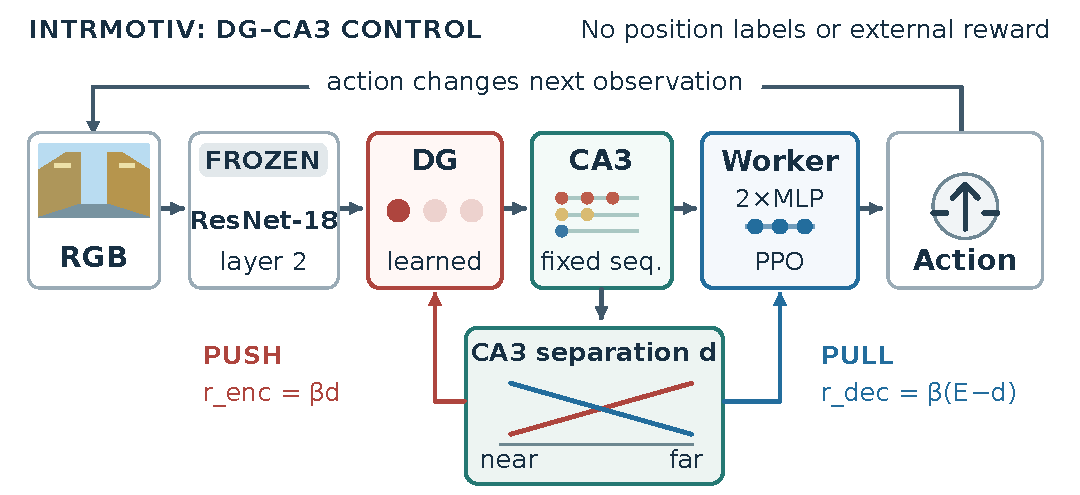
\includegraphics[width=\linewidth]{figures/architecture.pdf}
\captionof{figure}{\textbf{Author-supplied push--pull architecture.} A fixed ResNet-18 layer-2 visual trunk feeds a learned sparse DG layer (about 2.5\% active timesteps). Fixed CA3-like sequence dynamics carry DG events to the two-layer policy readout. Temporal separation gives DG its encoder credit (red); internally defined target encounters supply policy credit (blue). Actions determine the next observation.}
\label{fig:architecture}
\end{minipage}

\textbf{Representation and behavior.} Spatial DG activity rises during policy-driven exploration (Fig.~\ref{fig:results}A). On a common 10,001-observation replay, temporal DG credit increases the C01 DG spatial score in all five seed pairs (mean $+0.0575$), reduces map redundancy, and spreads eligible peaks over more arena area (Fig.~\ref{fig:results}B,E). Its effect reaches the readout: decoder-1 spatial information rises by $0.680$ bits per activation on average in all five C01 pairs (Fig.~\ref{fig:results}C). The C05 decoder-1 comparison mostly follows the same direction; C15 still has only three matched pairs.

\newpage
\textbf{Behavior and pull.} The policy selects the experiences through which this code is expressed. With weights frozen, each of the 38 available models evokes more informative decoder-1 activity under its own policy than under random actions (Fig.~\ref{fig:results}D). This action intervention establishes a behavioral expression effect. The temporal worker-hit bonus itself has mixed coverage and field effects against a constant hit bonus (Fig.~\ref{fig:results}F); a constant bonus still rewards target arrival, and actor--critic discounting still favors earlier arrivals. Longer PPO credit increases C15 coverage but reduces measured spatial information on separate policy rollouts. Commanded-target and physical-arrival results are still being analyzed.
% CHECK: The longer-credit comparison changes PPO gamma and GAE lambda jointly;
% its spatial maps follow separate policies. Do not call it isolated discounting.
% CHECK: Matched-command and physical-arrival evidence is pending; the compact
% worker panel is a placeholder, not evidence of improved goal following.

\begin{minipage}{\linewidth}
\centering
\begin{minipage}[c]{0.19\linewidth}\centering\textbf{A}\par
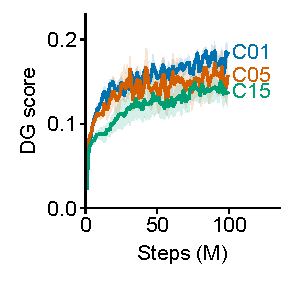
\includegraphics[width=\linewidth]{figures/online_spatial_course.pdf}\end{minipage}\hfill
\begin{minipage}[c]{0.46\linewidth}\centering\textbf{B}\par
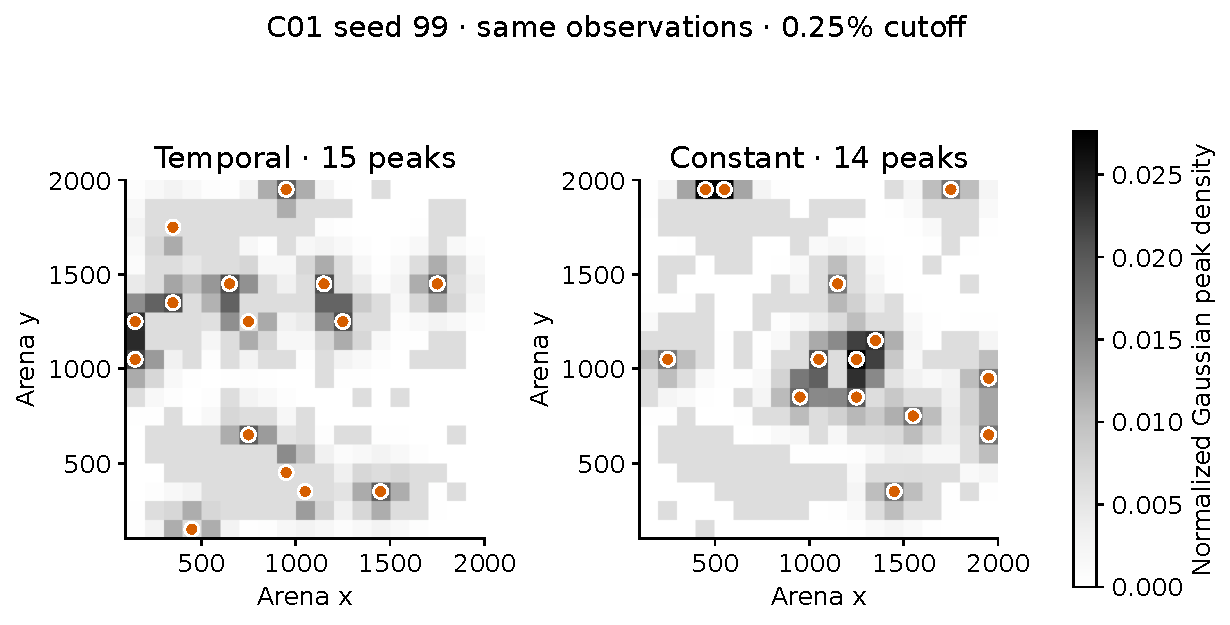
\includegraphics[width=\linewidth]{figures/c01_peak_density.pdf}\end{minipage}\hfill
\begin{minipage}[c]{0.32\linewidth}\centering\textbf{C}\par
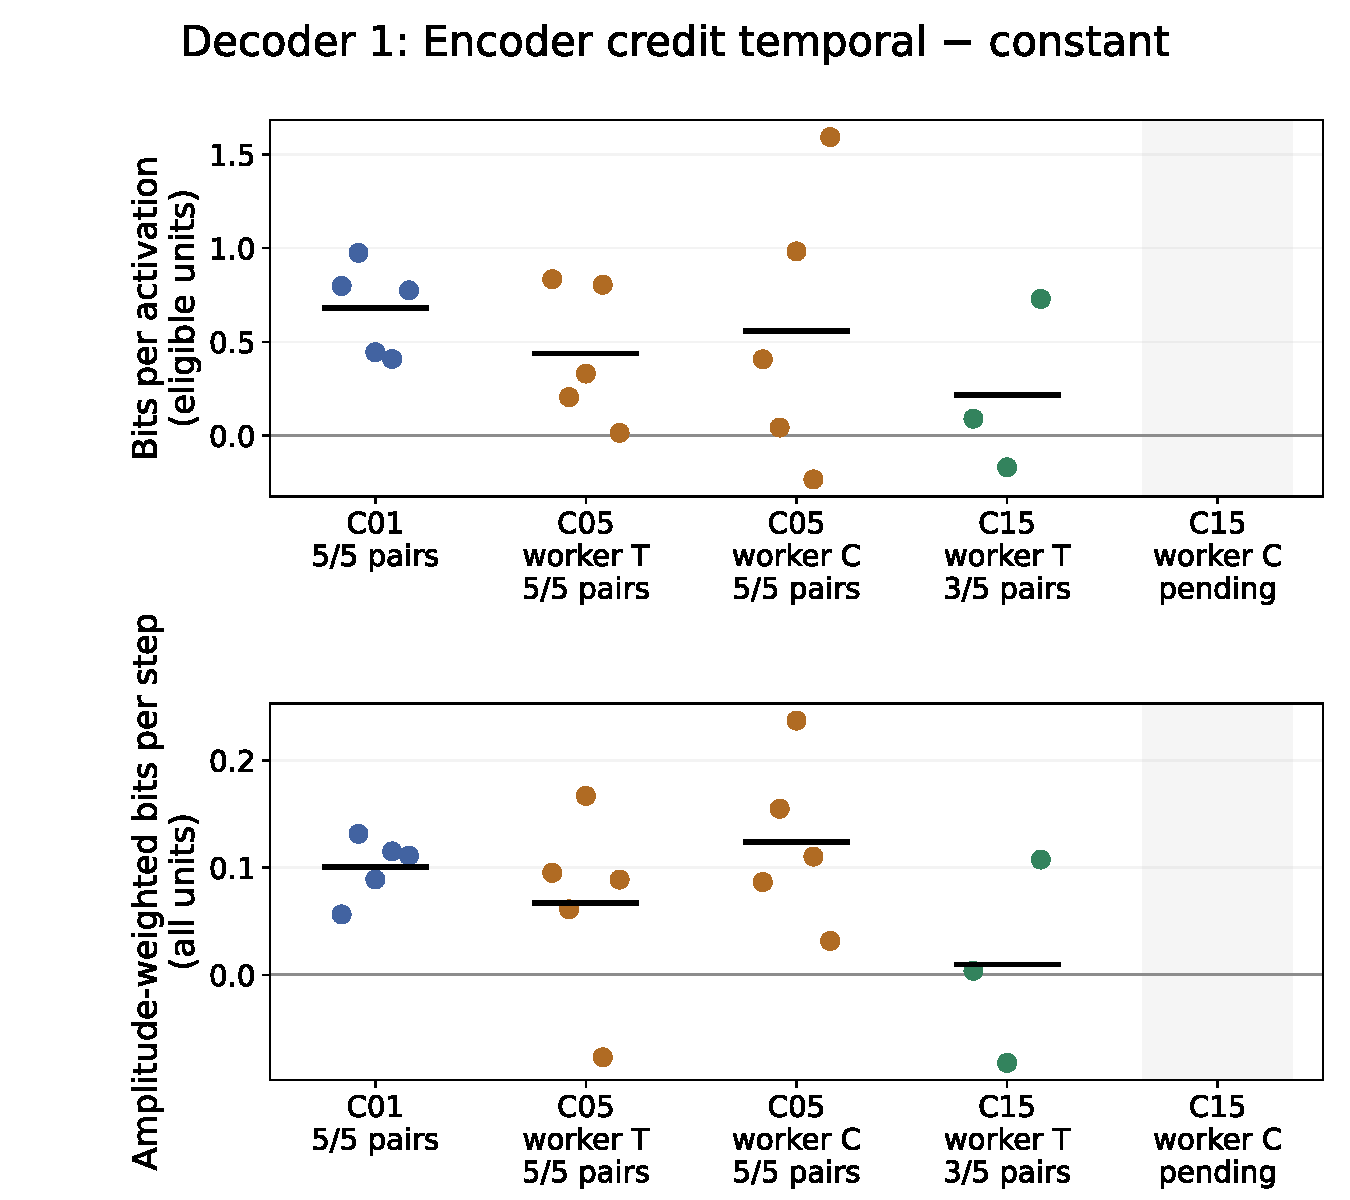
\includegraphics[width=\linewidth]{figures/encoder_paired_decoder_1.pdf}\end{minipage}
\par\vspace{2pt}
\begin{minipage}[t]{0.51\linewidth}\centering\textbf{D}\par
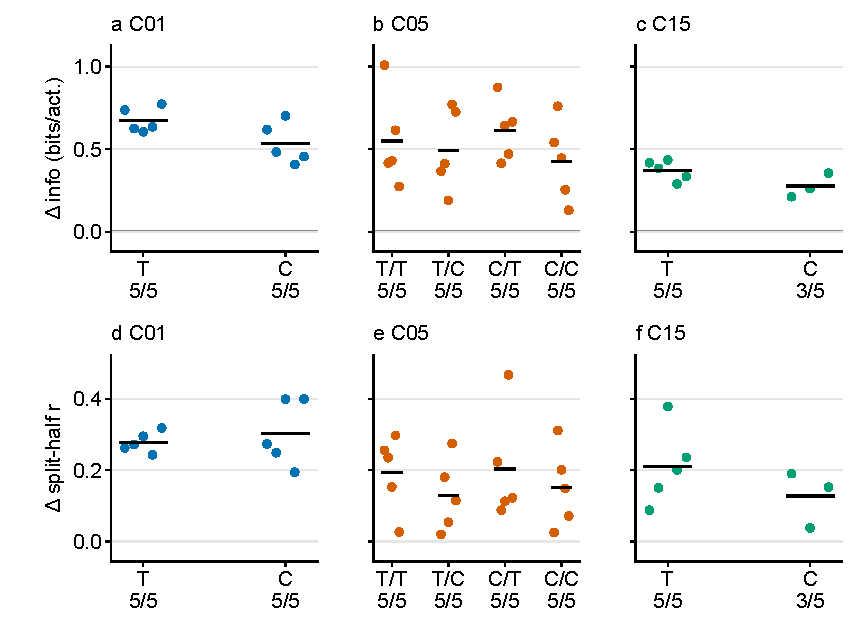
\includegraphics[width=\linewidth]{figures/behavior_expression_fresh.pdf}\end{minipage}\hfill
\begin{minipage}[t]{0.46\linewidth}\centering
\textbf{E}\par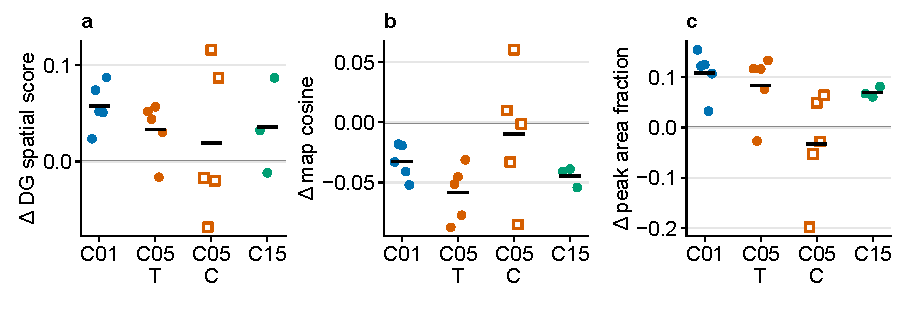
\includegraphics[width=\linewidth]{figures/encoder_credit_deltas.pdf}
\par\vspace{2pt}\textbf{F}\par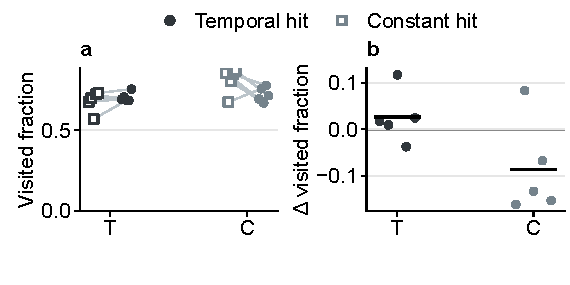
\includegraphics[width=0.82\linewidth]{figures/worker_coverage.pdf}
\end{minipage}
\captionof{figure}{\textbf{Spatial evidence in one panel set.} \textbf{A,} Online DG score, mean $\pm1$ s.e.m. across five seeds per temporal-credit family. \textbf{B,} C01 seed-99 peak-density example on the same 10,001 observations, temporal versus constant encoder credit; orange dots mark eligible peaks after a 0.25\% activity cutoff. \textbf{C,} Paired temporal-minus-constant decoder-1 information on that common panel; shaded C15 cells are pending. \textbf{D,} Own-policy minus random-action decoder-1 information and split-half reliability for 38 frozen models, with two repeats averaged per seed. \textbf{E,} DG spatial-score, map-similarity, and peak-area paired encoder contrasts on identical observations. \textbf{F,} Work in progress: C05 temporal versus constant worker-hit credit, showing last-window visited fractions and paired differences ($n=5$ per fixed encoder arm). Black bars mark seed means; T/C denote temporal/constant credit. Full-size source plots and analysis links are in the draft README.}
\label{fig:results}
\end{minipage}

\textbf{Comparison logic.} C01 isolates encoder timing without a worker target; C05 crosses encoder and worker timing in five matched seeds per arm, and C15 adds frontier goals, with three matched encoder seeds so far. The common replay fixes 10,001 external observations and action history, separating learned responses from evaluation paths. The own-versus-random probe instead fixes each network and changes actions. Together, these tests distinguish code formation from behavioral expression; matched-command analyses will determine whether worker credit improves target arrival.

\end{document}
